\documentclass[12pt]{article}
\usepackage[utf8]{inputenc}
\usepackage[left=2.5cm, right=2.5cm, top=2.0cm]{geometry}
\usepackage{sectsty}
\usepackage{graphicx}
\usepackage{amsmath}
\usepackage{amssymb}
% \usepackage{undertilde}
% \usepackage{kbordermatrix}
\usepackage{listings}
\usepackage{ulem}
\usepackage{soul}
% \usepackage{tikz}
% \usepackage{pgfplots}
% \pgfplotsset{compat=1.16}
\usepackage{siunitx}
\usepackage{pythonhighlight}
\usepackage{caption}
\usepackage{float}
\usepackage{url}
\usepackage{enumitem}
\usepackage{bm}
\usepackage{empheq}
\usepackage{tcolorbox}
\usepackage{framed}
\usepackage{xparse}
\usepackage{algorithm, algorithmic}
% \usepackage{algorithmic}
\usepackage{booktabs}
\usepackage{tabularx}
% ref packages
\usepackage{nameref}
% folowing  must be in this order
\usepackage{varioref}
\usepackage{hyperref}
\usepackage{cleveref}
\usepackage{mathtools}
\usepackage{longtable}
\DeclareMathOperator*{\argmax}{arg\,max}
% \usepackage[shortlabels]{enumitem}
\tcbuselibrary{breakable}
\allowdisplaybreaks


%  ---------------------- COMMANDS ---------------------------
% Double underline
\def\dunderline#1{\underline{\underline{#1}}}

% Shorten nonumber command
\def\nnb{\nonumber}

% Shorten boldsymbol command
\def\bs#1{\boldsymbol{#1}}

% Algorithmic newline
\def\algonewline{\STATE{ }}

% Eigenvectors of
\def\eigvecof{\text{eigenvectors of }}

% Eigenvalues of 
\def\eigvalof{\text{eigenvalues of }}

% Enclose in square brackets
\newcommand{\enclb}[1]{\left[#1\right]}
% Enclose in parenthesis
\newcommand{\enclp}[1]{\left(#1\right)}
% Enclose in curly brackets
\newcommand{\enclc}[1]{\left\{#1\right\}}

% Annotate first argument, text in second argument
\newcommand{\overtext}[2]{\overbrace{#1}^{\mathclap{\text{#2}}}}
\newcommand{\undertext}[2]{\underbrace{#1}_{\mathclap{\text{#2}}}}

% Normalization constant in multivariate normal
\newcommand{\mvnconst}[1]{\frac{1}{(2\pi)^{d/2} |#1|^{1/2}}}

% Exponential factor in multivariate normal
\newcommand{\mvnexpo}[3][x]{\exp \left[  -{\frac{1}{2}} (#1 - #2)^T #3^{-1} (#1 - #2) \right]}

% Multivariate normal
\newcommand{\mvn}[3][x]{\mvnconst{#3} \mvnexpo[#1]{#2}{#3}}

% For numbering in align* environment
\newcommand{\numberthis}{\addtocounter{equation}{1}\tag{\theequation}}

%  Sum notation w/ limits as argument and index as option
\newcommand{\sumlim}[3][i]{\sum\limits_{#1=#2}^{#3}}

%  Product notation w/ limits as argument and index as option
\newcommand{\prodlim}[3][i]{\prod\limits_{#1=#2}^{#3}}

%  Sum notation with only information beneath
\newcommand{\sumnolim}[1]{\sum\limits_{#1}}

%  Integral notation w/ limits as argument and index as option
\newcommand{\intlim}[2]{\int\limits_{#1}^{#2}}

%  Integral over whole domain notation, no args
\newcommand{\intinf}{\int\limits_{-\infty}^{\infty}}

%  Partial derivative notation, arg1: numerator, arg2: denominator
\newcommand{\pfrac}[3][ ]{\frac{\partial^{#1} #2}{\partial #3^{#1}}}

%  Derivative notation, arg1: numerator, arg2: denominator
\newcommand{\dvfrac}[3][ ]{\frac{\text{d}^{#1} #2}{\text{d} #3^{#1}}}

% When doing Gauss-Jordan, create arrow showing operations
\newcommand{\ro}[1]{\xrightarrow{\mathmakebox[\rowidth]{#1}}}

% ----------------------INVIRONMENTS---------------------------
% Item list with title
\newenvironment{titlemize}[1]{%
  \paragraph{#1}
  \begin{itemize}}
  {\end{itemize}}

  % Enum list with title
\newenvironment{titleenum}[1]{%
  \paragraph{#1}
  \begin{enumerate}}
  {\end{enumerate}}

  % Augmented matrix (matrix with vertical line)
\newenvironment{sysmatrix}[1]
  {\left(\begin{array}{@{}#1@{}}}
  {\end{array}\right)}

 % Make matrices with more spacing
\makeatletter
\renewcommand*\env@matrix[1][\arraystretch]{%
  \edef\arraystretch{#1}%
  \hskip -\arraycolsep
  \let\@ifnextchar\new@ifnextchar
  \array{*\c@MaxMatrixCols c}}
\makeatother

% \renewcommand*{\arraystretch}{1.5}

\newlength{\rowidth}% row operation width
\AtBeginDocument{\setlength{\rowidth}{3em}}

\floatname{algorithm}{Algorithm}
\renewcommand{\algorithmicrequire}{\textbf{Input:}}
\renewcommand{\algorithmicensure}{\textbf{Output:}}

\begin{document}
\title{\textbf{INF367A Project 2}}
\author{Naphat Amundsen}
\maketitle
\sectionfont{\fontsize{14}{15}\selectfont}
\subsectionfont{\fontsize{12}{15}\selectfont}
\subsubsectionfont{\fontsize{12}{15}\selectfont}
\graphicspath{ {./images/} }

\ifx
\begin{figure}[H]
	\centering
	\includegraphics[scale=0.8]{Figure_2}
	\caption{Insert caption here}
\end{figure}
\fi

\newcommand{\opGamma}{\operatorname{Gamma}}
\newcommand{\Um}{\underset{n \times k}{U}}
\newcommand{\Vm}{\underset{k \times m}{V}}

\section*{Introduction}
    This project is about creating a bayesian recommender engine specifically for movie ratings. There are different types of recommender systems. For this project, we will focus on \textit{collaborative filtering} where we try to predict user preferences based on preferences. We are given the MovieLens 100K dataset, which essentially consists of movies, users and the users ratings for the movies. The dataset contains $100 000$ ratings from $943$ users on $1682$ movies. The data is sparse, because not every user has rated every movie. The task is to predict the users ratings on movies that they have not seen. 

    The recommender system is based on Bayesian matrix factorization, that is, we want to predict ratings as well as estimating the uncertainty in the predictions. We try using three different models to estimate the matrix factors.

\section{The models}
    The user-rating pairs can be represented with the matrix $\underset{n \times m}{X}$, where each row represents a user, and each column represents as movie. To predict the users' rating on unreviewed movies, we try to factorize matrix into two matrices $\underset{n \times k}{U}, \underset{k \times m}{V}$ such that $UV \approx X$, where $k$ denotes the number of the latent dimensions of the factors. The matrices $U,V$ will be approximated using using Hamitonian Monte Carlo implemented in Stan \cite{HMC}.

    \subsection*{Data standard deviation}
        All the models share the same distribution for the data, that is $X_{ij}\sim N((UV)_{ij}, \beta)$. The prior for $\beta$ is chosen to be a gamma distribution with scale$=1$, and shape$=1$, which seems reasonable as we expect the data points to be close to whatever $UV$ estimates. Note that this is effectively an exponential distribution with rate $1$.
    
        \begin{figure}[H]
            \centering
            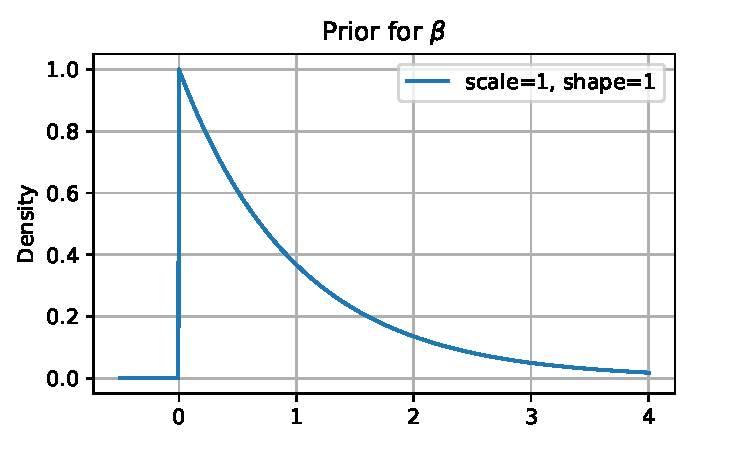
\includegraphics[width=0.5\textwidth]{betaprior.pdf}
            \caption{Probability density function for $\beta$, the assumed standard deviation of the data from the estimated values from $UV$.}
        \end{figure}
    
    \subsection{Normal model}
    This model is inspired from the "regular" way of doing Bayesian linear regression, that is the elements of $U$ and $V$ are normally distributed. To give more flexibility to the user, the normal distributions for $U$ and $V$ each has different sets of user specified parameters, that is the means and standard deviations. The data points is then assumed to be normally distributed, where the mean is what $UV$ is at the corresponding element, and the standard deviation assumed to be distributed by a gamma distribution with user specified values for shape and scale. The model should be reasonable, and should at least converge to some degree. 
    \begin{align*}
        U_{ij}  &\sim N(\mu_U, \sigma_U) \\
        V_{ij}  &\sim N(\mu_V, \sigma_V) \\
        \beta  &\sim \opGamma(a_\beta, b_\beta) \\
        X_{ij} &\sim N((UV)_{ij}, \beta) 
    \end{align*}

    User defined parameters: $\mu_U, \sigma_U, \mu_V, \sigma_V, a_\beta, b_\beta$.
    
    \vspace{3mm}
    We set the the means for the elemenets in $U$ and $V$ to be $0$, and set the standard deviations to be $5$, just to cover the range of the ratings within on standard deviation. That is: $\mu_U=0,\ \sigma_U=5,\ \mu_V=0,\ \sigma_V=5,\ a_\beta=1,\ b_\beta=1$.

    \subsection{Non-negative factorization model}
    The idea here is to constrain $U$ and $V$ to consist only of positive numbers, as the ratings are only positive after all. This model is very much like the normal model mentioned above, but the elements of $U$ and $V$ are gamma distributed instead.
    \begin{align*}
        U_{ij} &\sim \opGamma(a_U, b_U) \\
        V_{ij} &\sim \opGamma(a_V, b_V) \\
        \beta  &\sim \opGamma(a_\beta, b_\beta) \\
        X_{ij} &\sim N((UV)_{ij}, \beta) 
    \end{align*}

    User defined variables: $a_U, b_U, a_V, b_V, a_\beta, b_\beta$.
    
    \vspace{3mm}
    We specify the scale and shape such that the density "huddles" around $1$, as matrix multiplication will involve a lot of multiplications and additions when reconstructing $X$. We find it reasonable to expect values to not be very large. Specifically, the scale is $2$ and shape is $1$.
    \begin{figure}[H]
        \centering
        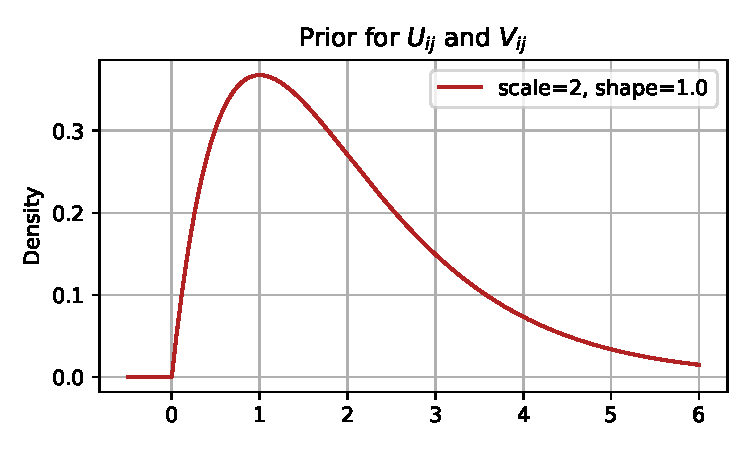
\includegraphics[width=0.5\textwidth]{nmfprior.pdf}
        \caption{Probability density function for the elements in $U$ and $V$.}
    \end{figure}
    To summarize: $a_U=2,\ b_U=1,\ a_V=2,\ b_V=1,\ a_\beta=1,\ b_\beta=1$.

    \subsection{ARD model}
    This model is inspired by the ARD (Automatic Relevance Determination) model used for regression tasks. This model can be viewed as an extension of the aforementioned "Normal model". The matrices $U$ and $V$ are still assumed to be distributed with gaussians. However, the difference is that each column (essentially components) of $U$ and $V^T$ has their own standard deviations. The standard deviations are assumed to be distributed from a gamma distribution with user specified parameters. We denote the standard deviations for the columns with the array $\alpha$ of size $k$, where each element correspond to each column of $U$ and $V^T$.
    \begin{align*}
        \alpha_{j}  &\sim \opGamma(a_\alpha, b_\alpha) \\
        U_{ij}  &\sim N(\mu_U, \alpha_j) \\
        V^T_{ij}  &\sim N(\mu_V, \alpha_j) \\
        \beta  &\sim \opGamma(a_\beta, b_\beta) \\
        X_{ij} &\sim N((UV)_{ij}, \beta)
    \end{align*}

    User defined variables: $\mu_U, \mu_V, a_\alpha, b_\alpha, a_\beta, b_\beta$.
    
    \vspace{3mm}
    We specify the same parameters as the Normal model for the ARD model where we can, that is the means and standard deviations for $U$ and $V$. We are unsure how the $\alpha$ values for the ARD should take, so we pick parameters for the prior distribution that does such that it does not assume much. 
    \begin{figure}[H]
        \centering
        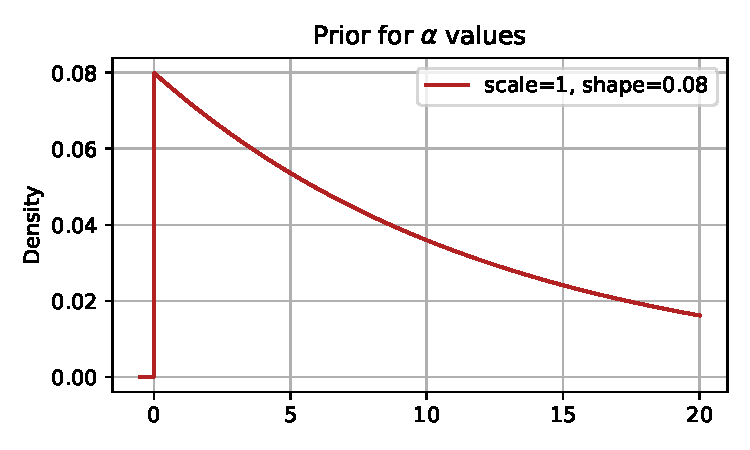
\includegraphics[width=0.5\textwidth]{alphaprior.pdf}
        \caption{Probability density for $\alpha$ values. Again, this is effectively equivalent to an expononential distribution. Note that the rate is quite low (compared to the one used for $\beta$).}
    \end{figure}
    To summarize the parameters for the ARD priors: $\mu_U=0,\ \sigma_U=5,\ \mu_V=0,\ \sigma_V=5,\ a_\alpha=1,\ b_\alpha=0.08, \ a_\beta=1,\ b_\beta=1$.

\section{Model selection}
We do model selection to find the best performing model on the dataset. There are many hyperparameters that can be tuned such as the scale and shape of gamma distributions for the $\beta$-value for the models. However, as the training time takes quite a while for each model, we limit the hyperparameter search to finding a good value for $k$, that is the latent dimension of the matrix factors $\underset{n \times k}{U}, \underset{k \times m}{V}$. 

After determining the best candidate on model the model selection, said candidate will be trained on $90\%$ of all the data, and then validated on the remaining $10\%$.

    \subsection{Data subsampling}
    To speed up the model selection process we do model selection on a subset of the data. We subsample 250 users and 250 movies. The matrix is sparse, so we want to subsample the data such that we get the "dense parts" of the matrix. To do this we pick the top 250 users based on number of movies rated, then we pick the top 250 movies with the most ratings from said users. This produces a $250 \times 250$ matrix with about $50\%$ observed elements. From the subset we create a train ($90\%$ of the subset) and a hold out set (the remaining $10\%$). The train set will be used for training, while the hold out set will be used for validation.

    \subsection{Model selection results}
    We try $1$ to $5$ latent dimensions for each model. We do 1200 iterations using Stan's HMC sampler, and set the "max\_treedepth" control argument to $15$ (the warnings from Stan told to) when sampling for each model.

        \subsubsection*{Scoring metric}
        To score the models we take the mean absolute error of all the predicted ratings to the actual ratings. That is, for each sampled $U$ and $V$, we get a corresponding $\hat{X}$, which contains predictions for the movie ratings. We calcuate the absolute error of the ratings contained in $\hat{X}$ to the ratings in the validation set. We do this for every sampled pairs of $U$ and $V$, and then we take the average error of all the calculated absolute errors. 
        
        % The algorithm is as follows:
        % \begin{algorithm}[H]
        %     \caption{mae, function to calculate mean absolute error given many sampled matrix factors $U$ and $V$. Note that the pseudo-code uses vectorized notation.}
        %     \label{alg:mae}
        %     \begin{algorithmic}[1]
        %         \REQUIRE {Us: sampled U factors, Vs: sampled V factors, row\_indices, column\_indices, ratings}
        %         \algonewline{}
        %         \STATE{// Us and Vs are 3D arrays, where each slice is a sampled U and V}
        %         \STATE{UVs $\leftarrow$ the corresponding U*V matrices to each U and V in Us and Vs}
        %         \algonewline{}
        %         \STATE{// Loop through the slices of UVs to obtain the predicted ratings for each}
        %         \STATE{// sampled U and V in Us and Vs}
        %         \STATE{preds $\leftarrow$ [UVs[row\_indices, col\_indices] for UV in UVs]}
        %         \algonewline{}
        %     \end{algorithmic}
        % \end{algorithm}
        % \begin{algorithm}[H]
        %     \caption{mae, function to calculate mean absolute error given many sampled matrix factors $U$ and $V$. Note that the pseudo-code uses vectorized notation.}
        %     \label{alg:mae}
        %     \begin{algorithmic}[1]
        %         \REQUIRE {Us: sampled U factors, Vs: sampled V factors, row\_indices, column\_indices, ratings, likelihood\_function}
        %         \algonewline{}
        %         \STATE{// Us and Vs are 3D arrays, where each slice is a sampled U and V}
        %         \STATE{UVs $\leftarrow$ the corresponding U*V matrices to each U and V in Us and Vs}
        %         \algonewline{}
        %         \STATE{// sample from the data likelihood function given Xs, since all the models use the same}
        %         \STATE{// likelihood function this is effectively $N(\text{(UV)}_{ij}, \vec{\beta})$}
        %         \STATE{// where $\vec{\beta}$ is the corresponding $\beta$ values for each slice of UVs.}
        %         \STATE{P $\leftarrow$ likelihood\_function.sample(UVs, $\ldots$)}
        %         \algonewline{}
        %         \STATE{P $\leftarrow$ likelihood\_function.sample(UVs, $\ldots$)}
        %     \end{algorithmic}
        % \end{algorithm}

    \begin{table}[H]
        \centering
        \caption{k is the latent dimension, train time shows training time in seconds, train MAE is the mean absolute error on the training set, while val MAE is the mean absolute error on the validation set. The table is sorted with respect to val MAE in ascending order.}
        \label{table:modelselection}
        \begin{tabular}{llrr|rr}
            \toprule
            {} &         model &  k &  train time (seconds) &  train MAE &  val MAE \\
            \midrule
            1  &           ARD &  3 &             3620.4200 &     0.6509 &   0.6822 \\
            2  &  Non-negative &  3 &             1437.8940 &     0.6499 &   0.6827 \\
            3  &        Normal &  3 &             1499.8993 &     0.6489 &   0.6828 \\
            4  &           ARD &  4 &             3774.4064 &     0.6414 &   0.6831 \\
            5  &           ARD &  2 &             2632.9194 &     0.6636 &   0.6845 \\
            6  &  Non-negative &  2 &             1375.8378 &     0.6631 &   0.6845 \\
            7  &        Normal &  2 &             1183.7930 &     0.6628 &   0.6850 \\
            8  &  Non-negative &  4 &             1920.2134 &     0.6408 &   0.6866 \\
            9  &           ARD &  5 &             4332.7366 &     0.6327 &   0.6881 \\
            10 &        Normal &  4 &             2712.8826 &     0.6385 &   0.6902 \\
            11 &  Non-negative &  5 &             1792.9489 &     0.6320 &   0.6934 \\
            12 &        Normal &  5 &             2775.1258 &     0.6283 &   0.6994 \\
            13 &        Normal &  1 &             1053.5344 &     0.6990 &   0.7082 \\
            14 &           ARD &  1 &             1549.5070 &     0.6992 &   0.7084 \\
            15 &  Non-negative &  1 &             1157.1555 &     0.6992 &   0.7084 \\
            \bottomrule
        \end{tabular}
    \end{table}
    
    \begin{table}[H]
        \centering
        \caption{This table shows the min, max, mean and standard deviation of the \textbf{Rhat} values from the sampling. The order of the rows correspond to Table \ref{table:modelselection}}
        \begin{tabular}{llr|rr|rr}
            \toprule
            {} &         model &  k &  Rhat min &  Rhat max &  Rhat mean &  Rhat std \\
            \midrule
            1  &           ARD &  3 &    0.9983 &    1.2125 &     1.0363 &    0.0625 \\
            2  &  Non-negative &  3 &    0.9983 &    1.1720 &     1.0197 &    0.0249 \\
            3  &        Normal &  3 &    0.9983 &    3.0460 &     1.4080 &    0.4549 \\
            4  &           ARD &  4 &    0.9983 &    2.7376 &     1.1919 &    0.3346 \\
            5  &           ARD &  2 &    0.9983 &    1.0476 &     1.0050 &    0.0085 \\
            6  &  Non-negative &  2 &    0.9983 &    1.0243 &     1.0017 &    0.0039 \\
            7  &        Normal &  2 &    0.9983 &    1.5620 &     1.1180 &    0.1400 \\
            8  &  Non-negative &  4 &    0.9983 &    3.0438 &     1.3131 &    0.3561 \\
            9  &           ARD &  5 &    0.9983 &    2.7210 &     1.2211 &    0.3202 \\
            10 &        Normal &  4 &    0.9983 &    3.0335 &     1.5988 &    0.5836 \\
            11 &  Non-negative &  5 &    0.9983 &    1.1397 &     1.0105 &    0.0183 \\
            12 &        Normal &  5 &    0.9983 &    1.9889 &     1.0930 &    0.1287 \\
            13 &        Normal &  1 &    0.9983 &    1.0325 &     1.0051 &    0.0045 \\
            14 &           ARD &  1 &    0.9983 &    1.3077 &     1.0821 &    0.0900 \\
            15 &  Non-negative &  1 &    0.9983 &    1.0282 &     1.0049 &    0.0045 \\
            \bottomrule
        \end{tabular}
    \end{table}
    
    \begin{table}[H]
        \centering
        \caption{This table shows the min, max, mean and standar deviation of the \textbf{N\_eff} (number of effective samples) values from the sampling. The order of the rows correspond to Table \ref{table:modelselection}}
        \begin{tabular}{llr|rr|rr}
            \toprule
            {} &         model &  k &  Neff min &  Neff max &  Neff mean &  Neff std \\
            \midrule
            1  &           ARD &  3 &    7.0254 & 1791.8795 &   371.5163 &  317.1653 \\
            2  &  Non-negative &  3 &   11.0431 & 1181.8516 &   193.7205 &  166.3506 \\
            3  &        Normal &  3 &    2.5894 &  736.3437 &    11.5601 &   21.9045 \\
            4  &           ARD &  4 &    2.9507 & 1404.7646 &   162.5089 &  202.3441 \\
            5  &           ARD &  2 &    5.3665 & 1533.4038 &   321.1908 &  333.7751 \\
            6  &  Non-negative &  2 &   19.9739 &  875.1028 &   184.0362 &  137.2979 \\
            7  &        Normal &  2 &    3.6549 &  880.2187 &    15.5561 &   31.7628 \\
            8  &  Non-negative &  4 &    2.6257 &  818.2812 &    59.7070 &   90.3463 \\
            9  &           ARD &  5 &    2.5573 &  876.6173 &    75.8097 &  108.1254 \\
            10 &        Normal &  4 &    2.5629 &  568.6558 &     7.9674 &   13.7378 \\
            11 &  Non-negative &  5 &   17.2196 & 1182.1601 &   153.6192 &   94.5881 \\
            12 &        Normal &  5 &    3.5170 &  687.1243 &    12.8534 &   15.9210 \\
            13 &        Normal &  1 &   15.9308 &  297.1190 &    37.1824 &   23.7075 \\
            14 &           ARD &  1 &    5.9032 &  589.1474 &    18.2738 &   27.6363 \\
            15 &  Non-negative &  1 &   30.8377 &  893.4888 &    73.1777 &   50.6046 \\
            \bottomrule
        \end{tabular}
    \end{table}

    The model selection process shows that the ARD model with $k=3$ is the best performer on the validation set. Concerning the convergence of the elements in the matrix factors, the Rhat may have a mean close to 1, but the standard deviation suggests that there is quite a spread for the values. The same goes for the number of efficient samples, where the mean in about $372$, but has a standard deviation of around $317$. The quick analysis of the number of effective samples and Rhat values suggests that not all elements in the matrix factors converged for said model. Nevertheless, the ARD
    model is still chosen to be the "best" candidate, based on the simple reasoning that it did manage to score the best on the
    validation set.

    \section{Evaluating the best model}
    We then try to train the best candidate from the model selection, that is the ARD model usng $3$ latent dimentions on a much larger amount of data. It should be noted that we effectively scrambled the data quite a bit during the early stages of experementing (we didn't seed in the beginning), thus we don't really have a proper test set, that is data that we have not touched whatsoever.
    
    \vspace{5mm}
    Using the whole dataset of $100000$ ratings, we create yet another train and validation set, where $90\%$ is used for the training set, and the rest for validation.

    \begin{figure}[H]
        \centering
        \caption{Credible intervals of 1500 elements from the predictive distribution. The firebrick-red dots are the means of predictive samples. The yellow dots are the true ratings. The elements correspond to the elements in the test-set.}
        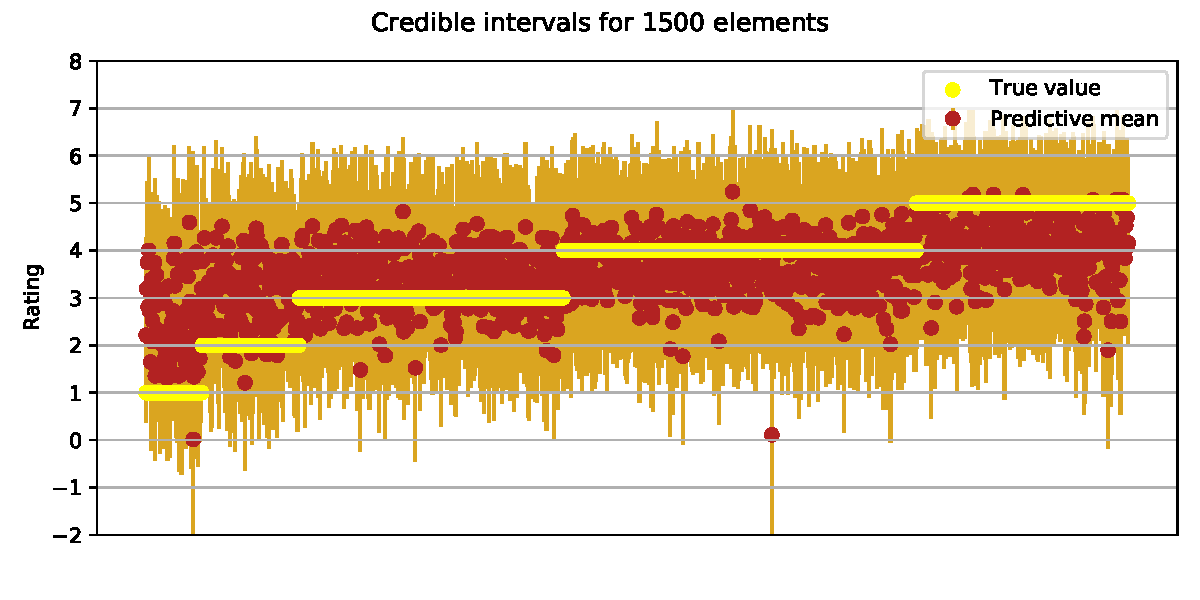
\includegraphics[width=\textwidth]{credibles.pdf}
    \end{figure}

% \bibliographystyle{apalike}
\bibliographystyle{ieeetr}
\bibliography{citations}

\end{document}
